\section{Produktfunktionen}
	% \input{3-Produktfunktionen}

		\subsection{Use Cases}
		% \input{3-1-Use_Cases}
		
		In dem zu modellierenden System wurden zwei Unterumgebungen (\emph{Server} sowie \emph{Robot Unit}) identifiziert, auf welchen die Aktoren \emph{Customer}, \emph{Hospital} und \emph{Robot Unit} verschiedene Anwendungsfälle aufrufen können. Der fiktionale Aktor \emph{User} aggregiert die gemeinsamen Use-Cases von \emph{Customer} und \emph{Hospital} \\
		%Die Abbildungen \ref{fig:3-1-server-use-cases} und \ref{fig:3-1-use-cases-robot-unit} stellen die Funktionalitäten dieser Teilsysteme dar.
			\subsubsection{Server}
			Der \emph{Server} stellt das zentrale System da, über welches die Aufträge der \emph{Customer} und des \emph{Hospitals} abgewickelt und an die \emph{Robots} verteilt werden.
				\begin{figure}[H]
					\centering
					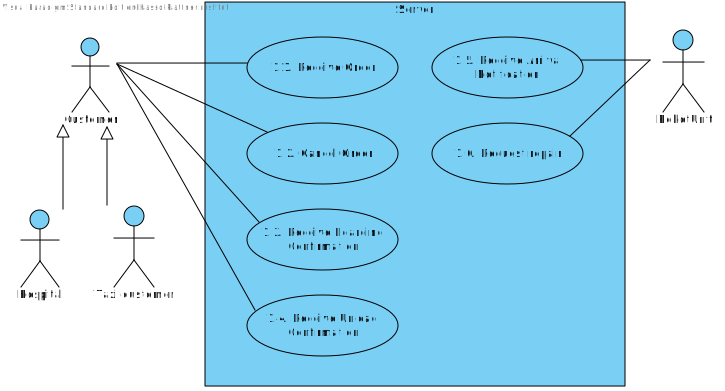
\includegraphics[width=0.8\textwidth]{img/2-Analyse-Server}
					\caption{Use Case Diagramm 1: Use Cases des Teilsystems \emph{Server}}
					\label{fig:3-1-server-use-cases}
				\end{figure}
			\pagebreak
			\subsubsection{Robot Unit}
			Die \emph{Robot Unit} stellt als Kombination des \emph{Robots} sowie der \emph{Robotsoftware} die ausführende Komponente dar und bietet dem Server Möglichkeiten der Steuerung und Informationsabfrage.
				\begin{figure}[H]
					\centering
					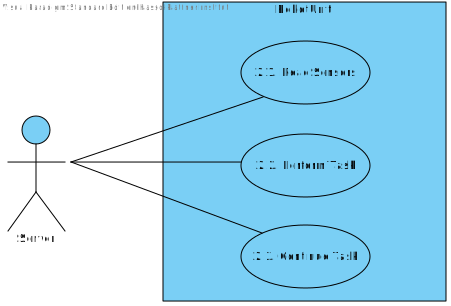
\includegraphics[width=0.8\textwidth]{img/2-Analyse-RobotUnit}
					\caption{Use Case Diagramm 2: Use Cases des Teilsystems \emph{Robot}}
					\label{fig:3-1-use-cases-robot-unit}
				\end{figure}

		\pagebreak

		\subsection{Beschreibungen der Use Cases in der \emph{Server} Umgebung}
			\subsubsection{Beschreibung zu Use Case \emph{1.1.}: Receive order}	
			\paragraph*{Charakterisierende Informationen}
			
			\begin{table}[H]
				\centering
				\begin{tabularx}{\textwidth}{|p{5cm}|X|}
					\hline
					\textbf{Übergeordneter elementarer Geschäftsprozess:} & TODO  \\ \hline
					\textbf{Ziel des Use Cases:} & \emph{Customer} können eine Anforderung (mit unterschiedlicher Dringlichkeit) an den \emph{Server} stellen. \\ \hline
					\textbf{Umgebende Systemgrenze:} & Server \\ \hline
					\textbf{Vorbedingung:} & \emph{Customer} verlangen ein Transportvehikel. \\ \hline
					\textbf{Nachbedingung bei erfolgreicher Ausführung:} & Auftrag wird ausgeführt. \\ \hline
					\textbf{Beteiligte Nutzer:} & \emph{Customer}, \emph{Server} und \emph{Robot Unit} \\ \hline
					\textbf{Auslösendes Ereignis:} & \emph{Customer} schickt einen konkreten Auftrag an den \emph{Server}. \\
					\hline
				\end{tabularx}
			\end{table}
			
			Über diesen Anwendungsfall können Aufträge und Anforderungen an den \emph{Server} durch Nutzer \emph{Customer} gestellt werden.
			Es findet eine Unterscheidung des anfragenden Nutzers statt, sodass Krankenfahrten priorisiert werden. \\ Sollte eine Fahrt auf Anfrage des Krankenhauses nicht sofort möglich sein, lehnt der \emph{Server} den Auftrag ab. Im Falle eines normalen Taxikunden (\emph{Customer}) wird der Auftrag, sofern kein \emph{Robot} bereit steht, in eine Warteschlange eingereiht.
			
				\paragraph*{Szenario für den Standardablauf (Erfolg)}
	
				\begin{table}[H]
					\centering
					\begin{tabularx}{\textwidth}{|c|p{2cm}|X|}
					\hline
					Schritt & Nutzer & Beschreibung der Aktivität \\ \hline
					1 & \emph{Customer}  & \emph{Customer} bestellen einen \emph{Robot} \\
					2 & \emph{Server} & \emph{Robot} fährt zum \emph{Customer}  \\
					\hline
					\end{tabularx}
				\end{table}
			\paragraph*{Szenarien für alternative Abläufe\\ (Misserfolg oder Umwege zum Erfolg)}	
					
			\begin{table}[H]
					\centering
					\begin{tabularx}{\textwidth}{|c|p{2cm}|X|}
					\hline
					Schritt & Bedingung für Alternative & Beschreibung der Aktivität \\ \hline
					1 & Es ist kein \emph{Robot} verfügbar & \emph{Server} lehnt beim \emph{Customer} den Auftrag ab bzw. gibt beim \emph{Customer} eine Warteschlange zurück \\
					\hline
					\end{tabularx}
				\end{table}
				
				
			
			%\paragraph*{Beschreibung des allgemeinen Ablaufes}
			
		
			
			\pagebreak
	
			\subsubsection{Beschreibung zu Use Case \emph{1.2.}: Confirm customer on board}
				\paragraph*{Charakterisierende Informationen}
				
				\begin{table}[H]
					\centering
					\begin{tabularx}{\textwidth}{|p{5cm}|X|}
						\hline
						\textbf{Übergeordneter elementarer Geschäftsprozess:} & TODO  \\ \hline
						\textbf{Ziel des Use Cases:} & Dem \emph{Server} signalisieren, dass ein \emph{Customer} in ein Taxi (\emph{Robot}) gestiegen ist. \\ \hline
						\textbf{Umgebende Systemgrenze:} & Gesamtsystem \\ \hline
						\textbf{Vorbedingung:} & Das Taxi (\emph{Robot}) erreicht den \emph {Customer} \\ \hline
						\textbf{Nachbedingung bei erfolgreicher Ausführung:} & Das Taxi (\emph{Robot}) setzt seine Fahrt mit zugestiegenem \emph{Customer} in Richtung dessen Ziel fort. \\ \hline
						\textbf{Beteiligte Nutzer:} & \emph{Customer} und \emph{Server} \\ \hline
						\textbf{Auslösendes Ereignis:} & Der \emph{Customer} bestätigt dem \emph{Server}, dass er in das Taxi (\emph{Robot}) eingestiegen ist. \\
						\hline
					\end{tabularx}
				\end{table}
				
				Der \emph{Customer} steigt in das Taxi ein und teilt dies dem \emph{Server} mit.
					\paragraph*{Szenario für den Standardablauf (Erfolg)}
	
				\begin{table}[H]
					\centering
					\begin{tabularx}{\textwidth}{|c|p{2cm}|X|}
					\hline
					Schritt & Nutzer & Beschreibung der Aktivität \\ \hline
					1 & \emph{Customer} & \emph{Customer} steigt in Taxi ein \\
					2 & \emph{Hospital} & \emph{Customer} teilt dem \emph{Server} mit, dass er eingestiegen ist \\
					\hline
					\end{tabularx}
				\end{table}
				
				%\paragraph*{Beschreibung des allgemeinen Ablaufes}
				
			\subsubsection{Beschreibung zu Use Case \emph{1.3.}: Check availability}
				\paragraph*{Charakterisierende Informationen}
				
				\begin{table}[H]
					\centering
					\begin{tabularx}{\textwidth}{|p{5cm}|X|}
						\hline
						\textbf{Übergeordneter elementarer Geschäftsprozess:} & TODO  \\ \hline
						\textbf{Ziel des Use Cases:} & Der \emph{Customer} erhält Auskunft über die Verfügbarkeit eines Taxis (\emph{Robot}) bzw. einer möglichen Wartelistenposition \\ \hline
						\textbf{Umgebende Systemgrenze:} & \emph{Server} \\ \hline
						\textbf{Vorbedingung:} & Der \emph{Customer} möchte ein Taxi bestellen. \\ \hline
						\textbf{Nachbedingung bei erfolgreicher Ausführung:} & Die Verfügbarkeit wird dem \emph{Customer} in der App angezeigt. \\ \hline
						\textbf{Beteiligte Nutzer:} & \emph{Customer} \\ \hline
						\textbf{Auslösendes Ereignis:} & \emph{Customer} stellt über App eine Anfrage an den \emph{Server} \\
						\hline
					\end{tabularx}
				\end{table}
				
				Nach Prüfen der Verfügbarkeit, kann der \emph{Customer} entscheiden, einen Auftrag abzusenden (\emph{Send order}). Falls nicht, ist keine weitere Interaktion mit dem \emph{Server} erforderlich.
				
				\paragraph*{Szenario für den Standardablauf (Erfolg)}
	
				\begin{table}[H]
					\centering
					\begin{tabularx}{\textwidth}{|c|p{2cm}|X|}
					\hline
					Schritt & Nutzer & Beschreibung der Aktivität \\ \hline
					1 & \emph{Customer} & \emph{Customer} sendet eine Anfrage an den \emph{Server} um die Verfügbarkeit eines Taxis zu überprüfen \\
					2 & \emph{Customer} & \emph{Customer} erhält Verfügbarkeitsinformationen \\
					\hline
					\end{tabularx}
				\end{table}
				
		
			\subsubsection{Beschreibung zu Use Case \emph{1.4.}: Cancel order}
				\paragraph*{Charakterisierende Informationen}
				
				\begin{table}[H]
					\centering
					\begin{tabularx}{\textwidth}{|p{5cm}|X|}
						\hline
						\textbf{Übergeordneter elementarer Geschäftsprozess:} & TODO  \\ \hline
						\textbf{Ziel des Use Cases:} & \emph{Customer} kann eine gestellte Anfrage an den \emph{Server} zurückziehen. \\ \hline
						\textbf{Umgebende Systemgrenze:} & \emph{Server}, \emph{Robot Unit} \\ \hline
						\textbf{Vorbedingung:} & Der \emph{Customer} überlegt sich, dass er die Bestellung eines Taxis stornieren möchte. \\ \hline
						\textbf{Nachbedingung bei erfolgreicher Ausführung:} & Der Auftrag wird gelöscht und der \emph{Robot} steht für andere Fahrten wieder zur Verfügung. \\ \hline
						\textbf{Beteiligte Nutzer:} & \emph{Customer} \\ \hline
						\textbf{Auslösendes Ereignis:} & Der \emph{Customer} storniert seine Bestellung eines Taxis. \\
						\hline
					\end{tabularx}
				\end{table}
				
				Der \emph{Customer} kann seine Bestellung eines Taxis solange stornieren, bis er zugestiegen ist.
				
				\paragraph*{Szenario für den Standardablauf (Erfolg)}
	
				\begin{table}[H]
					\centering
					\begin{tabularx}{\textwidth}{|c|p{2cm}|X|}
					\hline
					Schritt & Nutzer & Beschreibung der Aktivität \\ \hline
					1 & \emph{Customer} & \emph{Customer} zieht seinen Auftrag zurück \\
					\hline
					\end{tabularx}
				\end{table}
			
			\subsubsection{Beschreibung zu Use Case \emph{1.5.}: Inform about boarding}
				\paragraph*{Charakterisierende Informationen}
	
				\begin{table}[H]
					\centering
					\begin{tabularx}{\textwidth}{|p{5cm}|X|}
					\hline
					\textbf{Übergeordneter elementarer Geschäftsprozess:} & TakePatientToHospital   \\ \hline
					\textbf{Ziel des Use Cases:} & Dem \emph{Robot} mitteilen, dass Patient auf den \emph{Robot} geladen wurde \\ \hline
					\textbf{Umgebende Systemgrenze:} & \emph{Hospital} \\ \hline
					\textbf{Vorbedingung:} & Patient befindet sich auf \emph{Robot}\\ \hline
					\textbf{Nachbedingung bei erfolgreicher Ausführung:} & \emph{Robot} fährt Patienten zum \emph{Hospital} \\ \hline
					\textbf{Beteiligte Nutzer:} & \emph{Hospital}\\ \hline
					\textbf{Auslösendes Ereignis:} & \emph{Server} wurde informiert, dass \emph{Robot} am Patienten angekommen ist (\textit{ \glqq Inform about arrival \grqq }) \\
					\hline
					\end{tabularx}
				\end{table}
				
				Das \emph{Hospital} muss dem \emph{Robot} mitteilen, dass der \emph{Robot} mit dem \emph{Patient} beladen wurde, um einen sicheren Transport des Patienten zu gewährleisten. 
				Der \emph{Robot} hat somit keinen Eingriff in den Verladevorgang des Patienten.
	
				\paragraph*{Szenario für den Standardablauf (Erfolg)}
	
				\begin{table}[H]
					\centering
					\begin{tabularx}{\textwidth}{|c|p{2cm}|X|}
					\hline
					Schritt & Nutzer & Beschreibung der Aktivität \\ \hline
					1 & \emph{Hospital} & Patient wird auf Roboter beladen \\
					2 & \emph{Hospital} & \emph{Hospital} sendet Nachricht an Server, dass sich Patient auf dem \emph{Robot} befindet \\
					\hline
					\end{tabularx}
				\end{table}
	
		
			\subsubsection{Beschreibung zu Use Case \emph{1.6.}: Inform about unload}
				\paragraph*{Charakterisierende Informationen}
				
				\begin{table}[H]
					\centering
					\begin{tabularx}{\textwidth}{|p{5cm}|X|}
						\hline
						\textbf{Übergeordneter elementarer Geschäftsprozess:} & TakePatientToHospital  \\ \hline
						\textbf{Ziel des Use Cases:} & Den \emph{Server} informieren, dass Patient vom \emph{Robot} entfernt wurde \\ \hline
						\textbf{Umgebende Systemgrenze:} & \emph{Server} \\ \hline
						\textbf{Vorbedingung:} & \emph{Robot} ist am Ziel angekommen \\ \hline
						\textbf{Nachbedingung bei erfolgreicher Ausführung:} & Patient wurde erfolgreich vom \emph{Robot} entfernt und der \emph{Robot} steht für neue Aufgaben zur Verfügung \\ \hline
						\textbf{Beteiligte Nutzer:} & \emph{Hospital}, \emph{Server} \\ \hline
						\textbf{Auslösendes Ereignis:} & Patient wurde von Mitarbeitern des \emph{Hospitals} zur weiteren Behandlung abgeholt \\
						\hline
					\end{tabularx}
				\end{table}
				
				Dieser Use Case dient dazu, den \emph{Server} zu informieren, dass der Patient sicher vom \emph{Robot} entfernt wurde und dadurch wieder für neue Aufgaben zur Verfügung steht. 
				
				\paragraph*{Beschreibung des allgemeinen Ablaufes}
					\begin{table}[H]
					\centering
					\begin{tabularx}{\textwidth}{|c|p{2cm}|X|}
					\hline
					Schritt & Nutzer & Beschreibung der Aktivität \\ \hline
					1 & \emph{Hospital} & Patient wird vom Roboter entfernt \\
					2 & \emph{Hospital} & \emph{Hospital} sendet Nachricht an {Server}, dass Patient vom \emph{Robot} entfernt wurde \\
					\hline
					\end{tabularx}
				\end{table}
		
		\subsubsection{Beschreibung zu Use Case \emph{1.7}: Inform about arrival}

			\paragraph*{Charakterisierende Informationen}

			\begin{table}[H]
				\centering
				\begin{tabularx}{\textwidth}{|p{5cm}|X|}
				\hline
				\textbf{Übergeordneter elementarer Geschäftsprozess:} & TakePatientToHospital\\ \hline
				\textbf{Ziel des Use Cases:} & Ziel ist es, dem \emph{Robot} zu ermöglichen seine Ankunft dem Krankenhaus mitzuteilen\\ \hline
				\textbf{Umgebende Systemgrenze:} & \emph{Server}\\ \hline
				\textbf{Vorbedingung:} & Der \emph{Robot} erreicht die \emph{Position} des Patienten\\ \hline
				\textbf{Nachbedingung bei erfolgreicher Ausführung:} & Der \emph{Robot} wartet, bis er beladen wurde\\ \hline
				\textbf{Beteiligte Nutzer:} & \emph{Robot}\\ \hline
				\textbf{Auslösendes Ereignis:} & \emph{Robot} erreicht Patienten\\
				\hline
				\end{tabularx}
			\end{table}

			Der \emph{Robot} erreicht seine vorgegebene \emph{Destination} und muss dem \emph{Hospital} mitteilen, dass er angekommen ist. 

			\paragraph*{Szenario für den Standardablauf (Erfolg)}

			\begin{table}[H]
				\centering
				\begin{tabularx}{\textwidth}{|c|p{2cm}|X|}
				\hline
				Schritt & Nutzer & Beschreibung der Aktivität \\ \hline
				1 & Robot & \emph{Robot} informiert \emph{Server}, dass er angekommen ist. \\
				\hline
				\end{tabularx}
			\end{table}
				
				\pagebreak
		\subsection{Beschreibungen der Use Cases in der \emph{Robot Unit} Umgebung}
			\subsubsection{Beschreibung zu Use Case \emph{2.1.}: Read Sensors}
				
				\paragraph*{Charakterisierende Informationen}
				
				\begin{table}[H]
					\centering
					\begin{tabularx}{\textwidth}{|p{5cm}|X|}
						\hline
						\textbf{Übergeordneter elementarer Geschäftsprozess:} & Choose Robot\\ \hline
						\textbf{Ziel des Use Cases:} & \emph{Robot} kann über seinen Akkustand, seine Position und seine derzeitige \emph{Destination} Auskunft geben\\ \hline
						\textbf{Umgebende Systemgrenze:} & \emph{Robot Unit} und \emph{Server} \\ \hline
						\textbf{Vorbedingung:} & \emph{Robot} hat eine Anfrage vom \emph{Server} erhalten \\ \hline
						\textbf{Nachbedingung bei erfolgreicher Ausführung:} & \emph{Robot} schickt die ermittelten Informationen an den \emph{Server} \\ \hline
						\textbf{Beteiligte Nutzer:} & \emph{Robot} \\ \hline
						\textbf{Auslösendes Ereignis:} & \emph{Robot} hat eine Anfrage vom \emph{Server} erhalten, seine Sensoren zu lesen und sie dem \emph{Server} zu schicken \\
						\hline
					\end{tabularx}
				\end{table}
				
				Im Rahmen vom Geschäftsprozess \emph{Choose Robot} sammelt der \emph{Server}
				Informationen über jeden \emph{Robot}. Diese Informationen (z.B
				Akkustand, aktuelle Position, ob der \emph{Robot} gerade ein Ziel verfolgt)
				kann der \emph{Robot} von seinen Hardware-Schnittstellen anfordern. Dieser
				Use Case wird dann ausgefüht, wenn der \emph{Robot} eine Anfrage vom
				Server erhält, seine Sensoren zu lesen, und endet damit, dass der \emph{Robot}
				die zusammengefassten Informationen an den \emph{Server} schickt.
				
				\paragraph*{Szenario für den Standardablauf (Erfolg)}
				
				\begin{table}[H]
					\centering
					\begin{tabularx}{\textwidth}{|c|p{2cm}|X|}
						\hline
						Schritt & Nutzer & Beschreibung der Aktivität \\ \hline
						1 & Robot & \emph{Robot} erhält Anfrage vom \emph{Server} \\
						2 & Robot & \emph{Robot} sammelt Informationen von seiner Hardwareschnittstelle und fasst sie zusammen \\
						3 & Robot & \emph{Robot} schickt zusammengefasste Informationen an den Server \\
						\hline
					\end{tabularx}
				\end{table}
				
				%\paragraph*{Beschreibung des allgemeinen Ablaufes}
				
				\pagebreak
				
			\subsubsection{Beschreibung zu Use Case \emph{2.2.}: Assign Task}
				
				\paragraph*{Charakterisierende Informationen}
				
				\begin{table}[H]
					\centering
					\begin{tabularx}{\textwidth}{|p{5cm}|X|}
						\hline
						\textbf{Übergeordneter elementarer Geschäftsprozess:} & Choose Robot  \\ \hline
						\textbf{Ziel des Use Cases:} & \emph{Robot} den Task (die \emph{Destinations}) zuweisen\\ \hline
						\textbf{Umgebende Systemgrenze:} & \emph{Server} und \emph{Robot} \\ \hline
						\textbf{Vorbedingung:} & \textit{ \glqq Choose Robot \grqq } hat den am besten geeigneten \emph{Robot} gefunden und ausgewählt\\ \hline
						\textbf{Nachbedingung bei erfolgreicher Ausführung:} & Ausgewählter \emph{Robot} steuert die \emph{Destination} an\\ \hline
						\textbf{Beteiligte Nutzer:} & \emph{Server} und \emph{Robot}\\ \hline
						\textbf{Auslösendes Ereignis:} & Im Use-Case \textit{ \glqq choose Robot \grqq } wurde ein passender \emph{Robot} ausgewählt. Diesem soll nun die \emph{Task} übermittelt werden. \\
						\hline
					\end{tabularx}
				\end{table}
				
				Dem \emph{Server} wird hiermit die Möglichkeit gegeben, dem \emph{Robot} eine beliebige \emph{Destination} zuzuweisen. 
				
				\paragraph*{Szenario für den Standardablauf (Erfolg)}
				
				\begin{table}[H]
					\centering
					\begin{tabularx}{\textwidth}{|c|p{2cm}|X|}
						\hline
						Schritt & Nutzer & Beschreibung der Aktivität \\ \hline
						1 & Server & \emph{Server} überträgt ausgewähltem \emph{Robot} den Task \\
						\hline
					\end{tabularx}
				\end{table}
				
				%\paragraph*{Beschreibung des allgemeinen Ablaufes}
				
				\pagebreak
				
				
			\subsubsection{Beschreibung zu Use Case \emph{2.3.}: Continue Task}
			
			\paragraph*{Charakterisierende Informationen}
			
			\begin{table}[H]
				\centering
				\begin{tabularx}{\textwidth}{|p{5cm}|X|}
					\hline
					\textbf{Übergeordneter elementarer Geschäftsprozess:} & TODO  \\ \hline
					\textbf{Ziel des Use Cases:} & \emph{Robot} soll seinen Weg zur nächsten \emph{Destination} seines aktuellen \emph{Tasks} fortsetzen. \\ \hline
					\textbf{Umgebende Systemgrenze:} & \emph{Robot} und {Server} \\ \hline
					\textbf{Vorbedingung:} & \emph{Robot} hat seine aktuelle \emph{Destination} erreicht. \\ \hline
					\textbf{Nachbedingung bei erfolgreicher Ausführung:} & \emph{Robot} fährt seine nächste \emph{Destination} seines aktuellen \emph{Tasks} an. \\ \hline
					\textbf{Beteiligte Nutzer:} & \emph{Server} \\ \hline
					\textbf{Auslösendes Ereignis:} & \emph{Server} schickt konkrete Anweisung weiterzufahren an den \emph{Robot}. \\
					\hline
				\end{tabularx}
			\end{table}
			
			TODO
			
			%\paragraph*{Beschreibung des allgemeinen Ablaufes}
			
			\pagebreak
